% LaTeX Article Template - using color
\documentclass[11pt,a4paper]{exam}
%\documentclass[11pt,english,a4paper]{article}
% Load the "color" package
\usepackage{color}  %Gir farge?

\usepackage[utf8]{inputenc} %Gir ÆØÅ(?)
\usepackage{graphicx,textcomp,varioref} %ikke sikker

\usepackage{amsmath} %amsmatte
\usepackage{amsfonts} %amsmattefont
\usepackage{siunitx}
\usepackage{pdfpages}
\usepackage[colorlinks]{hyperref}
\usepackage{enumitem}

\usepackage{placeins}
\usepackage{epstopdf} %ikke sikker på om den trengs
\usepackage{subfigure} %selvforklarende
%\usepackage{url} %riktige url
\usepackage{float} % force figure to be HERE

\usepackage[backend=biber, bibencoding=utf8]{biblatex}
\bibliography{bibliography_AS7008.bib}

\usepackage{graphicx}
\graphicspath{% Tror ikke det er viktig
    {converted_graphics/}% inserted by PCTeX
}
\usepackage{helvet} %Times New Roman
%\usepackage{afterpage} %Times New Roman

\usepackage{tikz}  %Geometri
\usetikzlibrary{calc}
\usepackage{pifont}
\usepackage{threeparttable}%Gir bedre fotnoter
\usepackage{listings} %C++ kode
\usepackage{courier}
\lstset{basicstyle=\footnotesize\ttfamily,breaklines=true,language=python}
%
\begin{document}


\tolerance = 5000 % LaTeX er normalt streng når det gjelder linjebrytingen.
\hbadness = \tolerance % Vi vil være litt mildere, særlig fordi norsk har så
\pretolerance = 2000 % mange lange sammensatte ord.

\linespread{1.3} % linjeavstand enkel=1 halvannen=1.3 dobbel=1.6

%-------------------------------------------------------------------------
\newcommand{\ud}{\mathrm{d}} % definerer ny funksjon for å skrivedifferentialer
\renewcommand{\vec}[1]{\mathbf{#1}} % Tykke vektorsymboler
%\newcommand{\degree}{\ensuremath{^\circ}} %Gradsymbol
\long\def\symbolfootnote[#1]#2{\begingroup%
\def\thefootnote{\fnsymbol{footnote}}\footnote[#1]{#2}\endgroup} 


\firstpageheader{\bfseries\large FK7061 Statistical Methods in Physics\\Computer Lab 2}
{}
{\bfseries\large 28 Nov 2023\\ 
\href{mailto:pueh-leng.tan@fysik.su.se?Subject=FK7061}{\nolinkurl{pueh-leng.tan@fysik.su.se}}}
\runningheader{\bfseries FK7061 Statistical Methods in Physics}
{}
{\bfseries Autumn 2023}

\headrule
%--------------------------


%-------------------------------------Begynn dokument

\section*{Introduction}
In this computer lab, you will use Monte Carlo particle simulations made with the \texttt{Geant 4} package \footnote{\url{http://geant4.web.cern.ch/geant4/}}. You will explore the structure of the data, and perform some statistical calculations on them. 

\section{Programming preliminaries}
\subsection{Two-dimensional histograms}
Two-dimensional histograms are a good tool to explore correlations or distributions of your data. You can make one with \texttt{numpy} like this: 
\begin{lstlisting}
>>> import numpy as np
>>> import matplotlib.pyplot as plt
>>> xs = np.array([1,5,3,5,2])
>>> ys = np.array([0,4,2,3,1])
>>> #NOTE THE ORDER OF X AND Y:
>>> H,xbin,ybin =np.histogram2d(ys,xs,bins=5)
>>> xmin = xbin[0]
>>> xmax = xbin[-1]
>>> ymin = ybin[0]
>>> ymax = ybin[-1]
>>> im = plt.imshow(H,extent=[xmin,xmax,ymin,ymax],origin='low',cmap=plt.cm.afmhot)
>>> plt.show()
\end{lstlisting}

\subsection{Finding percentiles of a numpy array}
It is convenient to be able to quickly determine percentiles of a \texttt{numpy} array: 
\begin{lstlisting}
 >>>> import numpy as np
 >>>> x = np.array([0,5,3,2,5])
 >>>> #10percentile:
 >>>> print( np.percentile(x,10))
0.8
 >>>> #75percentile:
 >>>> print( np.percentile(x,75))
5.0
\end{lstlisting}
\subsection{concatenating numpy arrays}
The example below shows how you can concatenate two \texttt{numpy} arrays: 
\begin{lstlisting}
>>> import numpy as np
>>> a = np.array([[1,2],[3,4]])
>>> b = np.array([[5,6],[7,8]])
>>> c = np.concatenate([a,b])
>>> print( c)
[[1 2]
 [3 4]
 [5 6]
 [7 8]]
\end{lstlisting}

\subsection{Finding all files matching a pattern}
Using \texttt{glob}, you can find all files matching a pattern: 
\begin{lstlisting}
>>> import glob
>>> glob.glob('*.txt')
['emailFK706116.txt', 'Exercises.txt', 'labAttendance16.txt']
\end{lstlisting}

\subsection{Interpolating a function}
You can interpolate from a function using \texttt{scipy.interpolate.interp1d}.

\begin{lstlisting}
>>> import matplotlib.pyplot as plt
>>> from scipy import interpolate
>>> x = np.arange(0, 10)
>>> y = np.exp(-x/3.0)
>>> f = interpolate.interp1d(x, y)

>>> xnew = np.arange(0, 9, 0.1)
>>> ynew = f(xnew)   # use interpolation function returned by `interp1d`
>>> plt.plot(x, y, 'o', xnew, ynew, '-')
>>> plt.show()
\end{lstlisting}

\section{Physics Introduction}
\subsection{Particles through matter}
Relativistic charged particles traversing matter lose energy in three main ways:\footnote{For an overview of particle
detection, \emph{Detectors for Particle radiation} by Konrad Kleinknecht was the lab tutors choice this time.}
\begin{enumerate}[start=1]
    \item The particle may ionize atoms, kicking out an electron. This effect dominates at low energies. 
    \item The particle may emit transition radiation at a material boundary
    \item The particle may radiate photons through e.g. Cherenkov radiation or Bremsstrahlung. This is the largest effect at the highest energies, and is inversely proportional to the particle's mass.
\end{enumerate}
At high energies ($E>5$ MeV), the dominant effect for photons is the creation of an $e^+e^-$ pair. As particles create photons through bremsstrahlung, a high-energy electron or photon will create an $e^+e^-$ pair, resulting in more relativistic electrons radiating photons that pair-produce etc. Electrons or photons will therefore both create a large "Electromagnetic Shower" at high enough energies.
\begin{figure}[H]
    \centering
        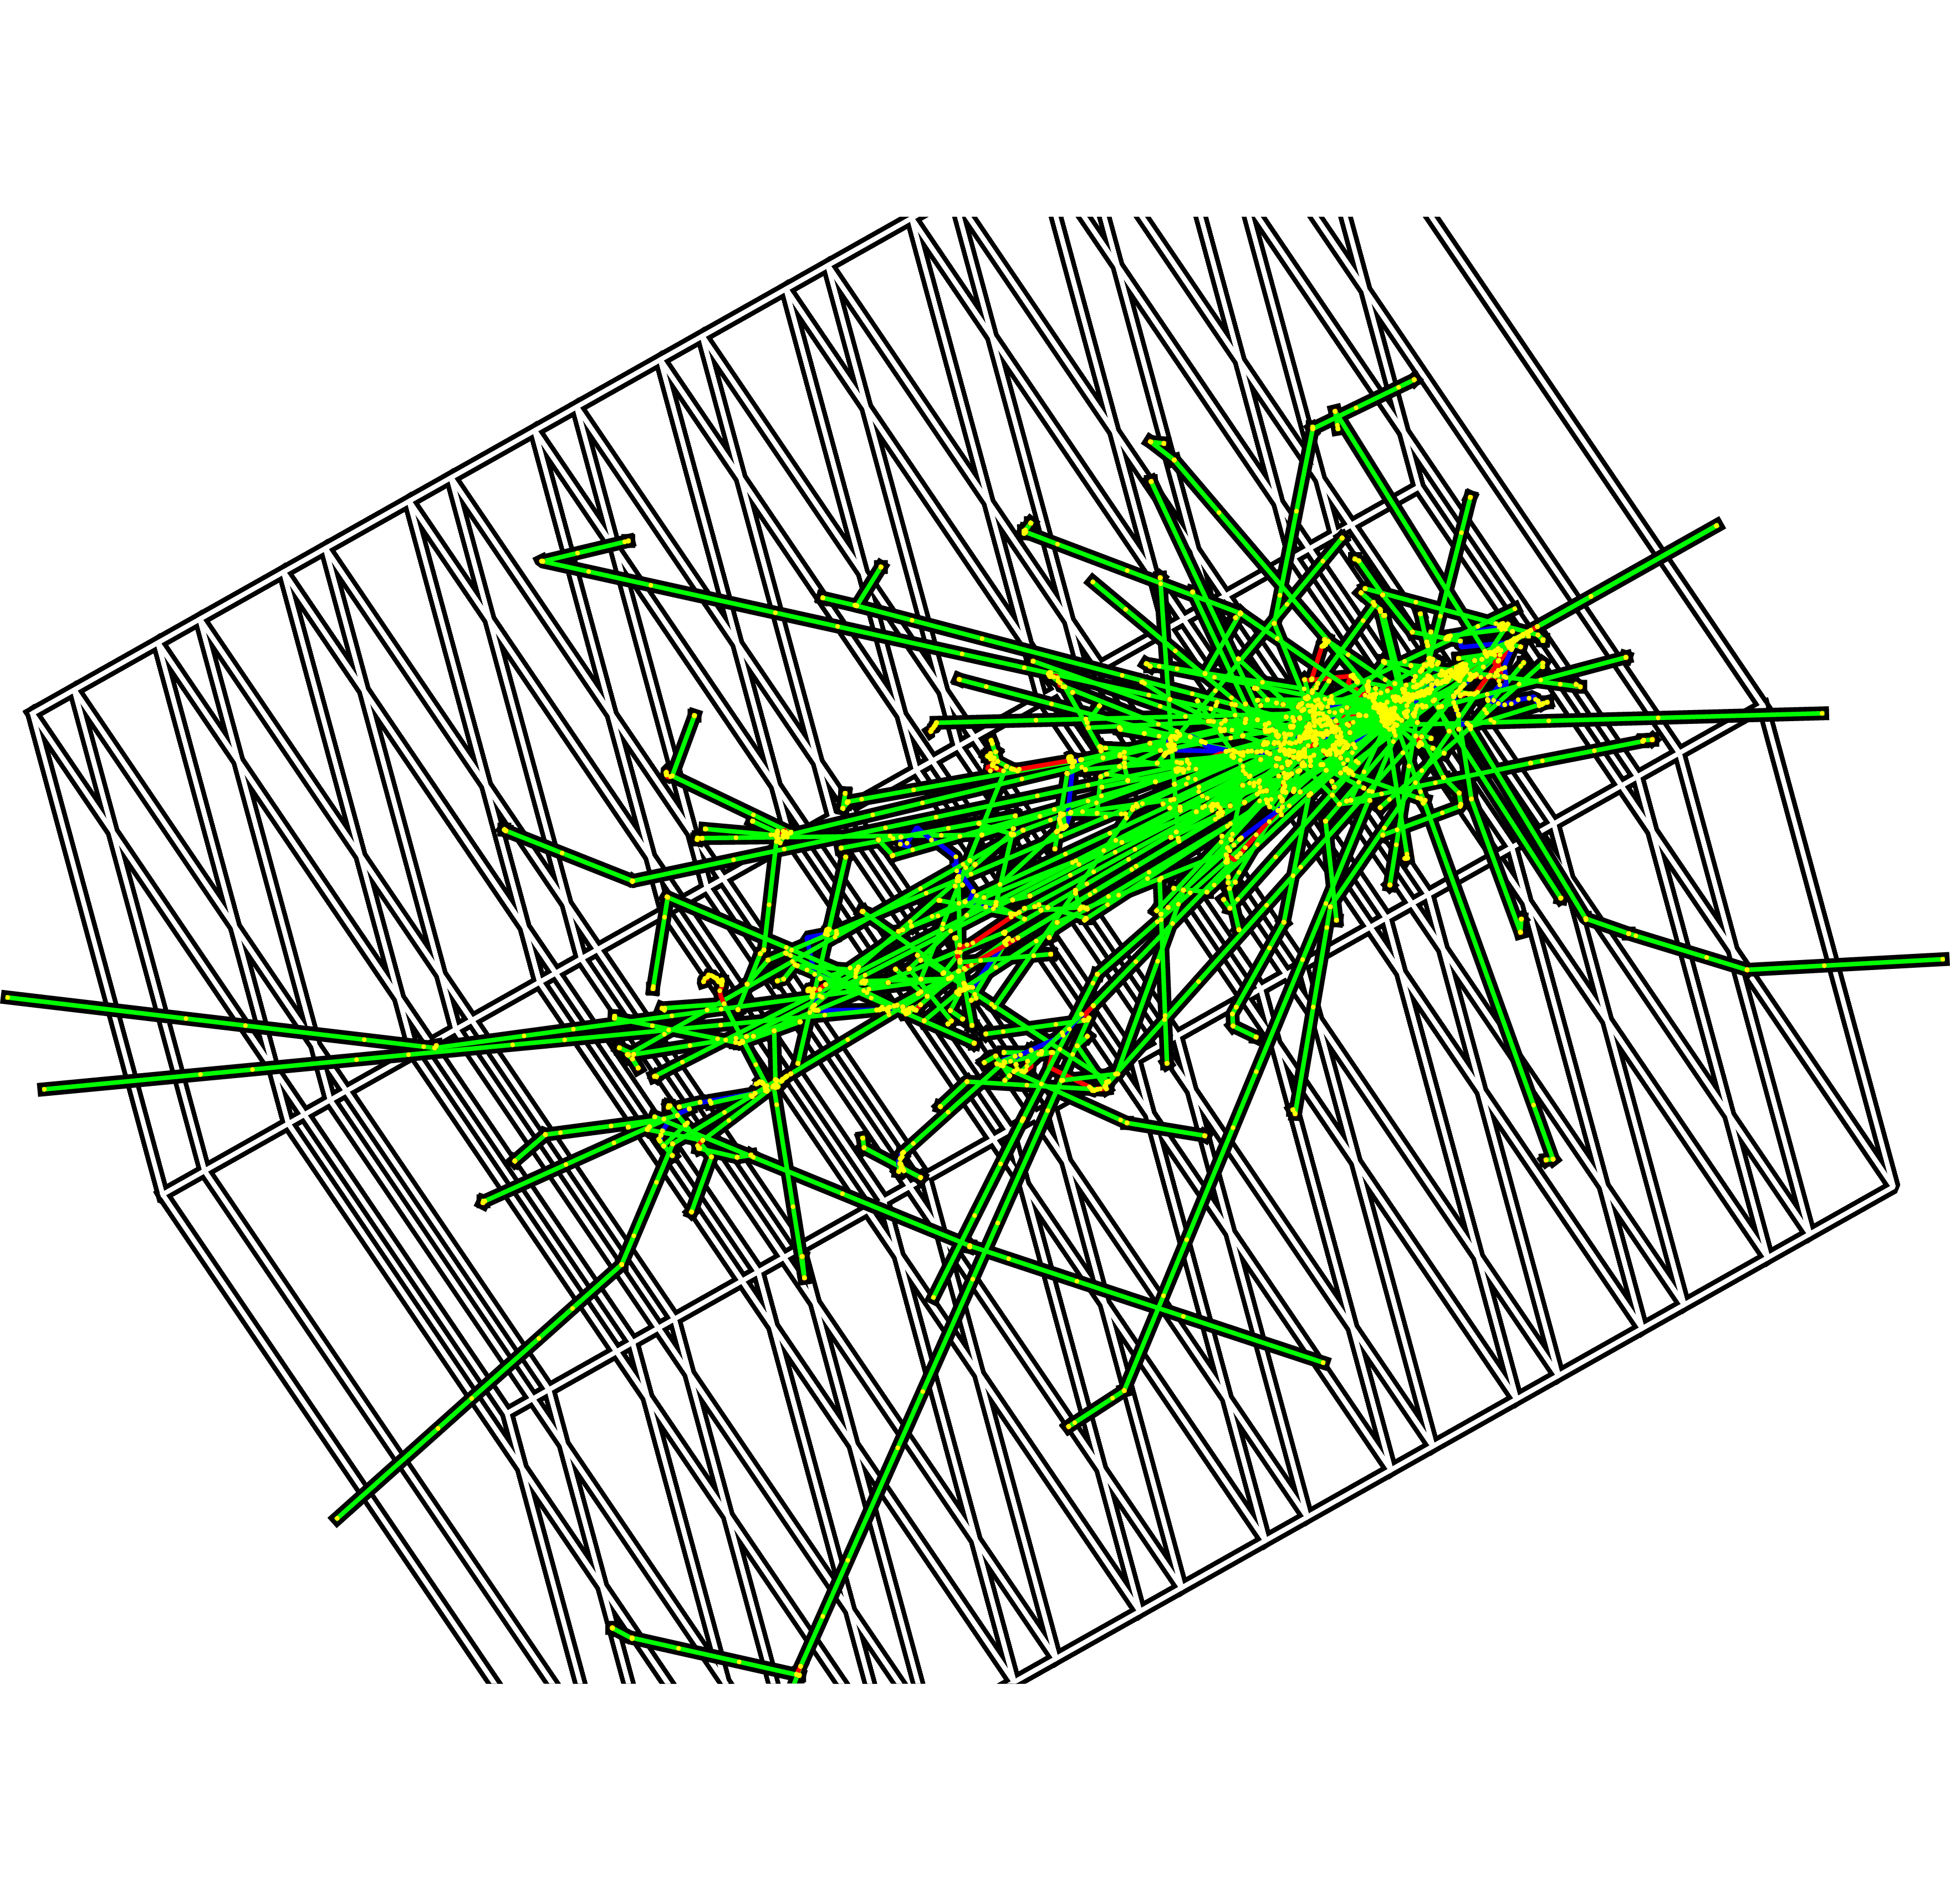
\includegraphics[height=3in]{gammashower.png}
    \caption{Electromagnetic shower in calorimeter induced by a photon}
    \label{fig:gamma}
\end{figure}
In contrast, muons, which are $~200$ times heavier than electrons, radiate less, and will interact much less with matter. Particle physics detectors typically identify muons this way; any charged particle that passes through the entire detector without losing much energy is classified as a muon.
\begin{figure}[H]
    \centering
        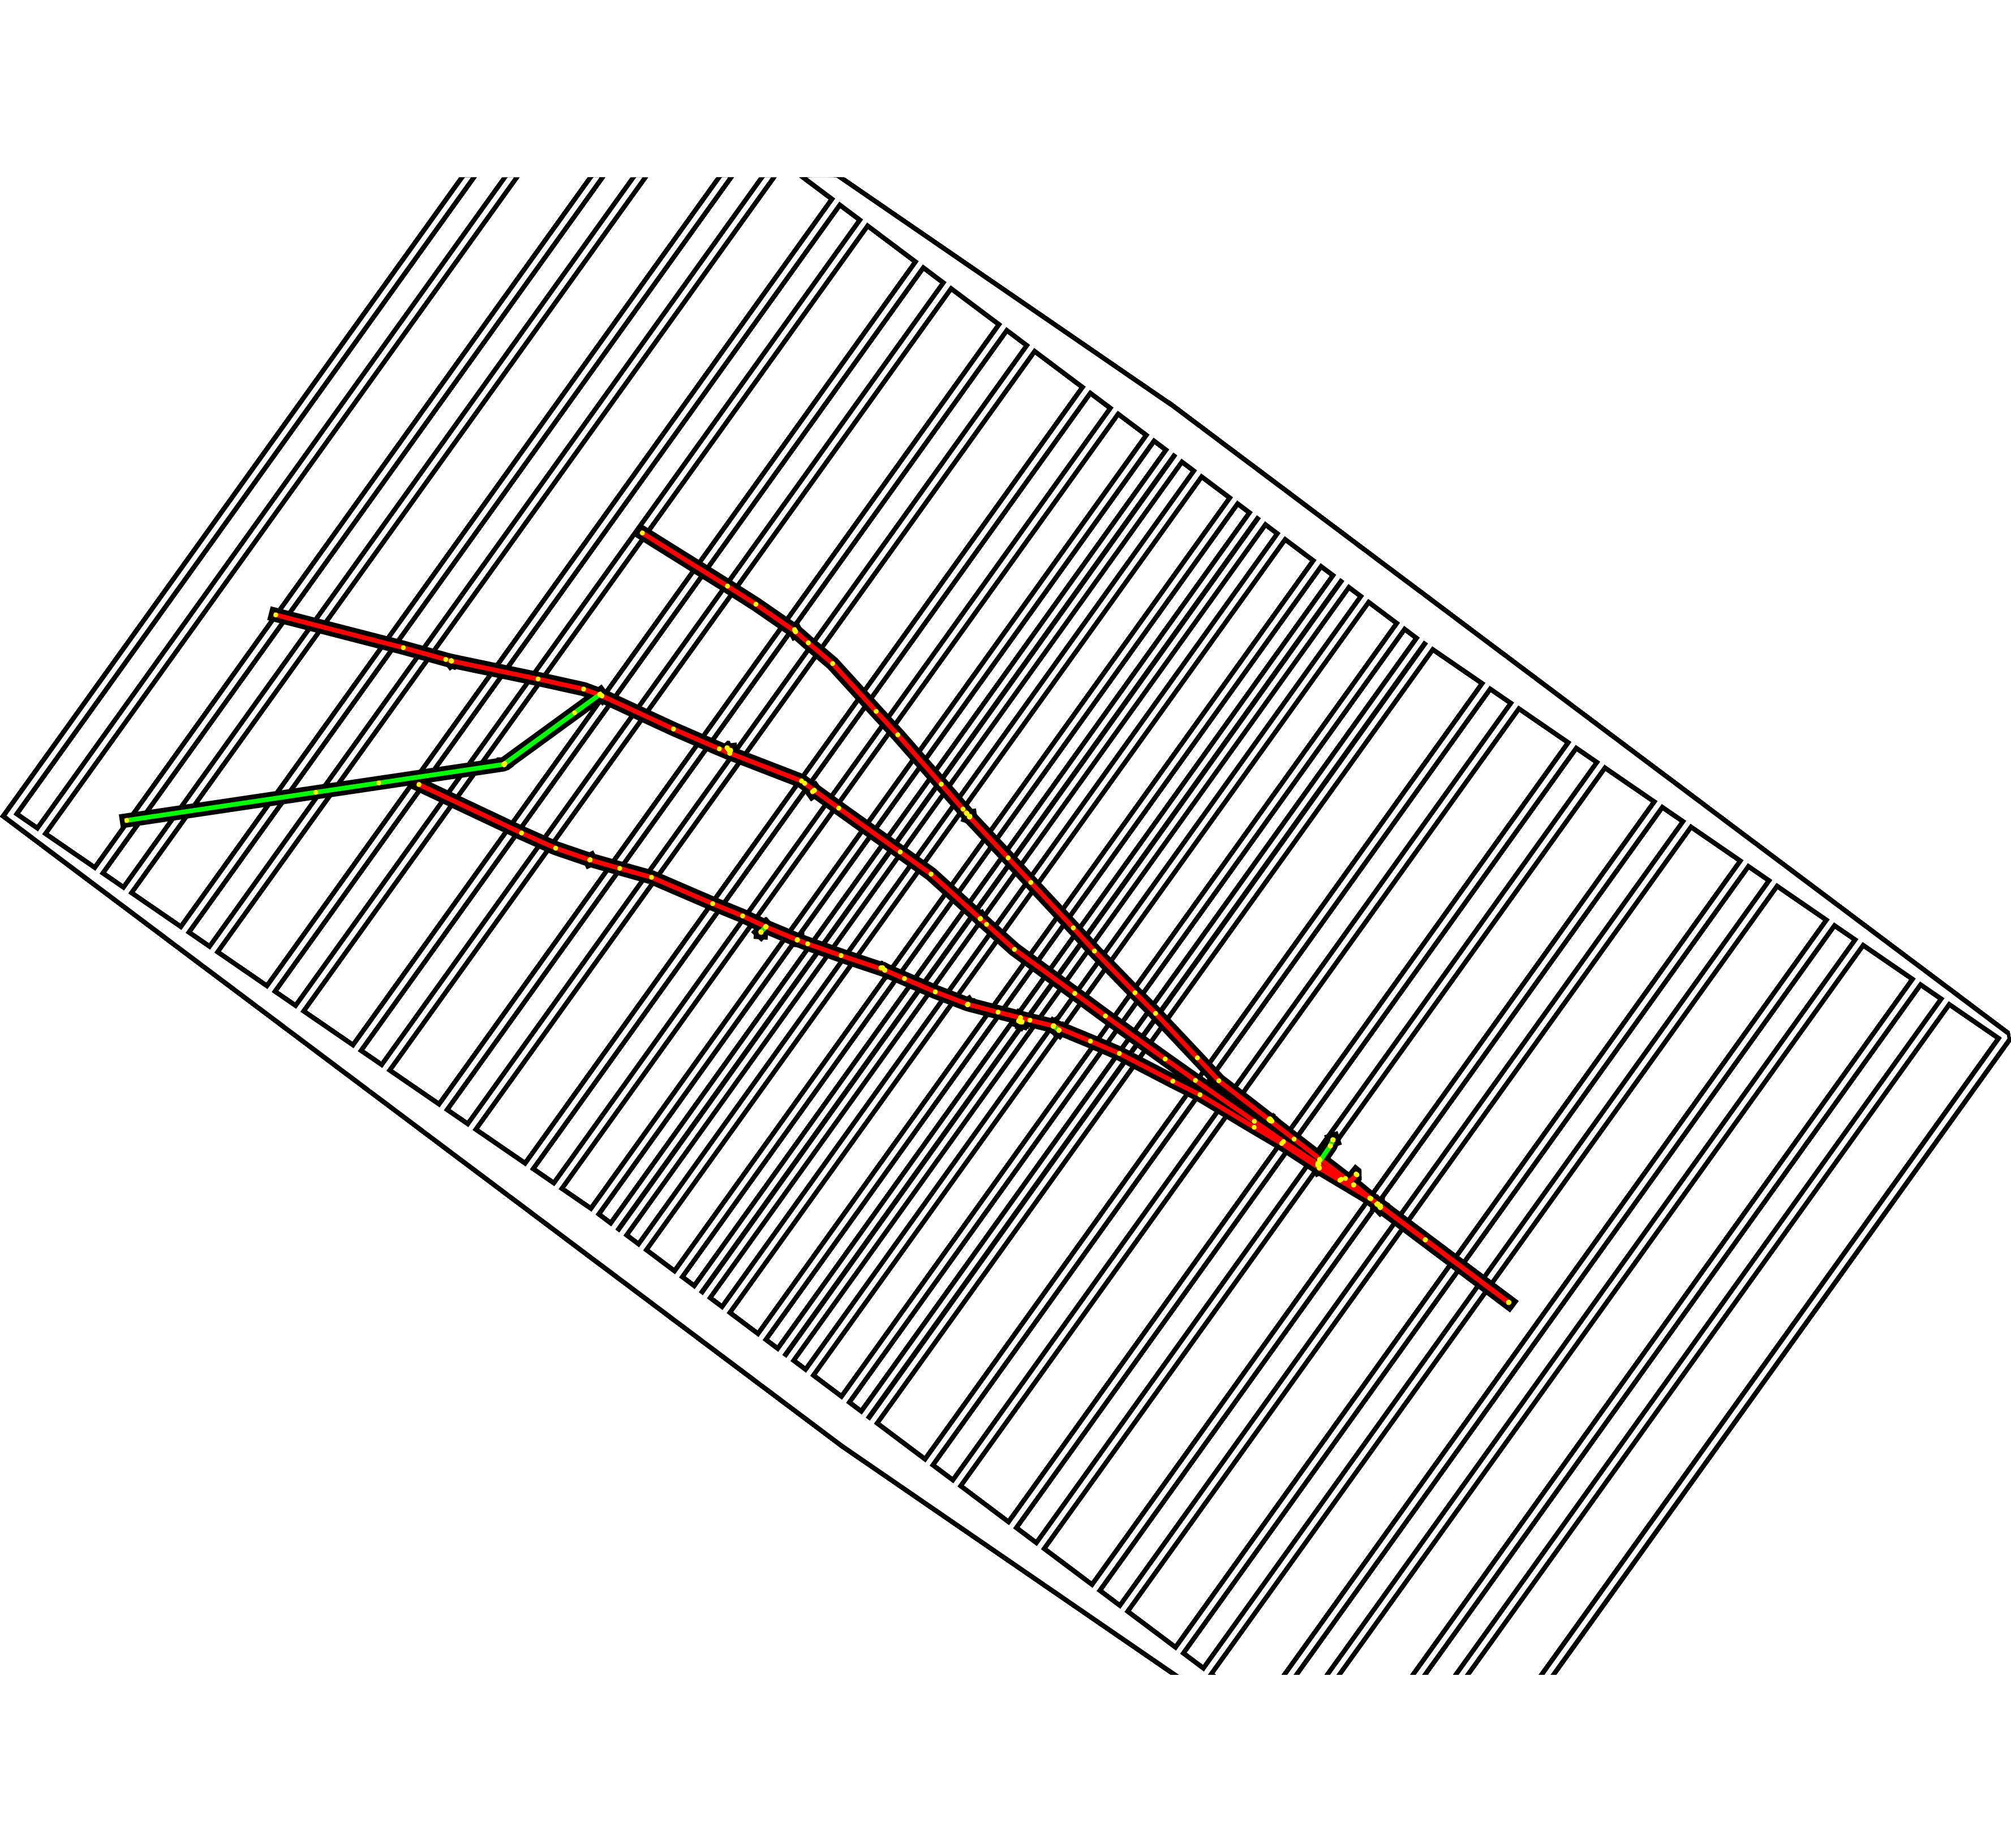
\includegraphics[height=3in]{muonshower.png}
    \caption{Muon creating a couple of secondary electrons in the calorimeter. The particles bend because of the magnetic field.}
    \label{fig:muon}
\end{figure}

\subsection{Reading the data}
The data you are given is saved in \texttt{numpy}'s \texttt{.npy} format. Each file contains an array, with five numbers for each event, and can be loaded like this: 

\begin{lstlisting}
>>>> import numpy as np
>>>> a = np.load("numpyfile.npy")
>>>> a.shape
(5030, 5)
>>>> print( a[0])
[125.48915443   10.00555455  109.60118788   51.44653892  100.        ]
\end{lstlisting}

In order, the numbers are: 
\begin{enumerate}[start=0]
    \item $E_{abs}$; The energy (in $MeV$) deposited in the absorbing lead plates.  
    \item $E_{gap}$; The energy (in $MeV$) deposited in the argon gas.
    \item $L_{abs}$; The total length (in $mm$) of all particle tracks in the absorbing lead plates. 
    \item $L_{gap}$; The total length (in $mm$) of all particle tracks in the argon gas. 
    \item $E_{true}$; The true initial energy (in $MeV$) of the incoming particle. 
\end{enumerate}
Of these numbers, we typically measure only the energy and total track length in the argon gas\footnote{These calorimeters are therefore called \emph{sampling} calorimeters}. We wish to reconstruct the initial energy of the incoming particle, or alternatively, we wish to use $E_{gap}$ as an estimator of the total deposited energy, $E_{dep}=E_{abs}+E_{gap}$. For simplicity, you may assume in this lab that we can measure $E_{abs}$ and $L_{abs}$ with negligible measurement error. Three sets of files are provided where the original particle is an electron, a muon or a photon, respectively, with energies between $1000$ MeV and $2000$ MeV. The file names reflect the contents of the files. For instance, \texttt{RunNtup\_e-\_1000\_Etru\_1000.00.npy} contains MC electron events at 1000 MeV.

\subsection{Calorimeters}
In this exercise, you will be given files for a lead-argon calorimeter. This technique is widely used, for example in the ATLAS detector. $10mm$ plates of lead absorb the shower, while the calorimeter read out in $5mm$ gaps between the plates. Charged shower particles traversing the liquid argon filled gap ionize the liquid, which can be read out. The energy deposited in the liquid argon is roughly equal to the sum of the length of all the particle tracks in the gap.
\begin{itemize}
    \item Pick a subset of the simulated events from the file labelled \texttt{RunNtup\_HighStatistics*.npy} and plot a scatter plot of the total deposited energy against the total track length for the electrons, the photons, and the mystery sample. What do you observe?
\end{itemize}

\subsection{Monte Carlo simulation}
A particle moving through matter has a probability (depending on density, material, particle type  etc.) to interact in different ways. \texttt{Geant4} has physics lists - a table of every interaction that is implemented. Below, you see a couple as printed in the output file: 
\begin{lstlisting}
eIoni:   for  e-    SubType= 2
      dE/dx and range tables from 100 eV  to 10 TeV in 77 bins
      Lambda tables from threshold to 10 TeV, 7 bins per decade, spline: 1
      finalRange(mm)= 1, dRoverRange= 0.2, integral: 1, fluct: 1, linLossLimit= 0.01
      ===== EM models for the G4Region  DefaultRegionForTheWorld ======
        MollerBhabha :  Emin=        0 eV    Emax=       10 TeV

eBrem:   for  e-    SubType= 3
      dE/dx and range tables from 100 eV  to 10 TeV in 77 bins
      Lambda tables from threshold to 10 TeV, 7 bins per decade, spline: 1
      LPM flag: 1 for E > 1 GeV,  HighEnergyThreshold(GeV)= 10000
      ===== EM models for the G4Region  DefaultRegionForTheWorld ======
             eBremSB :  Emin=        0 eV    Emax=        1 GeV   DipBustGen
            eBremLPM :  Emin=        1 GeV   Emax=       10 TeV   DipBustGen
\end{lstlisting}
The sheer number of interactions, the multiple detector geometries, etc. mean that we must turn to Monte Carlo
methods to compute e.g. the distributions of positrons that transverse some complex piece of matter\footnote{say your head in a PET scanner, or, if you are unlucky, in a synchrotron}.

\begin{itemize}
\item Can you think of some statistical distributions needed to simulate elementary particles?
\end{itemize}

\section{Lab task}
\subsection{Showers vs. MIPs}
\begin{itemize}
    \item Open up some of the files, and plot the histograms of the deposited energy in lead and in the gas gap for the various particles. How are they different? If you had to tell the difference between muons and electrons, could you do it? 
    \item If yes, imagine you have found $N=15$ particles you are sure to be muons after running your experiment an hour. What are your upper and lower limits on the expected number of muons per hour at a 90\% confidence level?
\end{itemize}

\subsection{Estimating electron fraction}
Look at the files with \texttt{HighStatistics} in their filenames. They contain $10^5$ events of photons and electrons with $100$ MeV and $200$ MeV incident energy respectively. Suppose you wish to find out how many photons there are compared to electrons.
\begin{itemize}
    \item  With this high-statistic data set, how would you estimate the probability density function for $L_{gap}$ for each of the two species of particles?
    \item What is the expression of the likelihood function for this data set? Hint: You would need to include the number of electrons, photons, PDF for $L_{gap}$ for electrons, photons, and remember that you do not always observe the exact number of events you expect from your model.
    \item Construct the likelihood function for the number of photons and electrons using the mystery MC events in \verb|mystery_Etru_-1.00.npy|, and compute the maximum likelihood estimate of the number of photons and electrons in the mystery sample.
\end{itemize}


%---------------------------------------------END Document----------------------------
\end{document}

